%!TEX root = ../dissertation.tex


\chapter{\label{chap:basics}Neutrinos and Neutrino Oscillations}




Neutrinos and anti-neutrinos are particles produced in many nuclear reactions such as beta decays,
\begin{equation}
{}^A_Z X \to {}_{Z+1}^AX + e^- +\bar \nu_e .
\end{equation}
In such reactions, charged current weak interaction plays a role which takes a down quark in neutron to a up quark while releasing electrons and anti-electron neutrino,
\begin{equation}
n\to p + e^- + \bar \nu_e .
\end{equation}
More generally, positron emission and electron capture are also neutrino-related nuclear reactions which is explained in table \ref{table:Neutrino_Reactions}. In the context of astrophysics, (anti)neutrinos also participate in nuclear reaction chains in stars, synthesis of heavy and rare elements and more. I will summarize the properties of neutrinos and some relevant astrophysical problems.

\begin{table}[ht]
\centering
 \begin{tabular}{|c | c | c|} 
 \hline
 Reaction & Equation & Boson   \\ [0.5ex] 
 \hline
 Electron emission & ${}^A_Z X \to {}^A_{Z+1}X + e^- +\bar \nu_e$ & $W$  \\ 
 Positron emission & ${}^A_Z X \to {}^A_{Z-1}X + e^+ + \nu_e$ & $W$  \\
 Electron capture & ${}^A_Z X + e^- \to {}^A_{Z-1}X  + \nu_e$ &  $W$ \\
 Positron capture & ${}^A_Z X + e^+ \to {}^A_{Z+1}X  + \bar\nu_e$ &  $W$ \\
 [0.5ex] 
 \hline

 Electron annihilation &  $e^- + e^+  \to \nu_e + \bar\nu_e $  & $W$ \\
 Electron annihilation &  $e^- + e^+  \to \nu + \bar\nu $  & $Z$ \\
 [0.5ex] 
 \hline

  Neutrino capture & ${}^A_{Z}X + \overset{(-)}{\nu_e} \to {}^A_{Z\mp 1}X + e^\pm $ & W\\
  [1ex] 
 \hline
 $e^-\nu$ scattering & $e^- + \overset{(-)}{\nu_e} \to e^- + \overset{(-)}{\nu_e} $ &  $W$ \\
 $e^-\nu$ scattering & $e^{\pm} + \overset{(-)}{\nu_e} \to e^{\pm} + \overset{(-)}{\nu_e} $ &  $Z$ \\
 Neutrino scattering & $ {}^A_Z X + \overset{(-)}{\nu} \to {}^A_Z X + \overset{(-)}{\nu} $ &  Z\\
 [0.5ex] 
 \hline
 \end{tabular}
 \caption{Neutrino related nuclear or leptonic reactions}
\label{table:Neutrino_Reactions}
\end{table}





\section{\label{chap:basics-section:neutrinos}Neutrinos as Fundamental Particles}

Neutrinos are fundamental particles in standard model of particle physics. I summarize some of the properties that is useful in this thesis in Table~\ref{table:neutrino-properties}.

\begin{table}[ht]
\centering
 \begin{tabular}{|c | c | c|} 
%  \hline
%  Property & Equation & Boson   \\ [0.5ex] 
 \hline
  Electric Charge & 0\\
  \hline
  Spin & $1/2$ \\
\hline
 Mass & $<2\mathrm{eV}$  \\
 \hline
 Interactions & Weak, Gravitation  \\
 \hline
 Flavors & $\nu_e$, $\nu_\mu$, $\nu_\tau$ \\ 
 \hline
 Chirality & Left \\
 \hline
 Hypercharge & $-1$ \\
 \hline
 
 \end{tabular}
 \caption{Properties of Neutrinos~\cite{Patrignani:2016xqp}}
\label{table:neutrino-properties}
\end{table}

\section{\label{chap:basics-section:astro}Stars as Neutrino Factories}

Astrophysical neutrino sources such as cores of stars, AGN, Gamma-ray bursts, and supernovae, reveals a lot of information about the sources. Though neutrinos are are weakly interacting particles rendering them hard to detect, it is an important subject to theoretically inspect neutrino productions in astrophysical processes.


\subsection{Stellar Core}

One of the neutrino factories is the stellar core. Numerous nuclear reactions as well thermal neutrino production produce luminous neutrinos. In this section, the nuclear reactions in stars are reviewed as well as the neutrino oscillations in the stars.

% \begin{figure}[ht]
% \centering
% 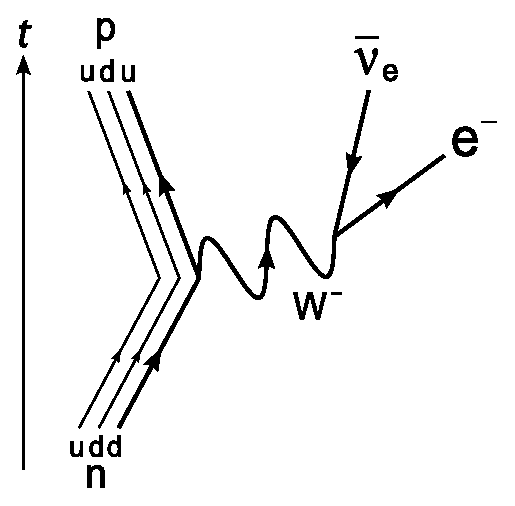
\includegraphics{chapters/assets/solar/Beta_Negative_Decay.eps}
% \caption{Feynman diagram of beta decay. The charged current weak interaction boson in this case is a $W^-$. Credit: Joel Holdsworth, licensed under public domain.}
% \label{fig:Beta_Negative_Decay}
% \end{figure}

\subsection{Nuclear Reactions in Sun and Solar Neutrino Flux}

The most important nuclear reactions in our Sun are pp chain and CNO cycle. Through different stages of its life, a star experience different nuclear reactions. Figure \ref{fig:pp_Chain_Branching} shows the dominant energy source of solar mass stars. In order to calculate the neutrino spectrum we need the neutrino production rate in each reaction and the branching ratios. The processes that emits neutrinos are the reactions in red in Fig~\ref{fig:pp_Chain_Branching}, which are~\cite{Altmann2001}
\begin{align}
&\mathrm{p+p\to {}^2H + e^+ +\nu_e},  & \mathrm{\leq 0.422MeV}\\
&\mathrm{{}^7Be + e^- \to {}^7Li + \nu_e} , &\text{0.862MeV for 90\%}\\
&&\qquad \text{0.384MeV for 10\%} \\
&\mathrm{{}^8B \to {}^8Be^* +e^+ +\nu_e},  & \mathrm{\leq 15 MeV}
\end{align}




\begin {figure*}%[!hbtp]
\centering
\begin{adjustbox}{width=\textwidth}
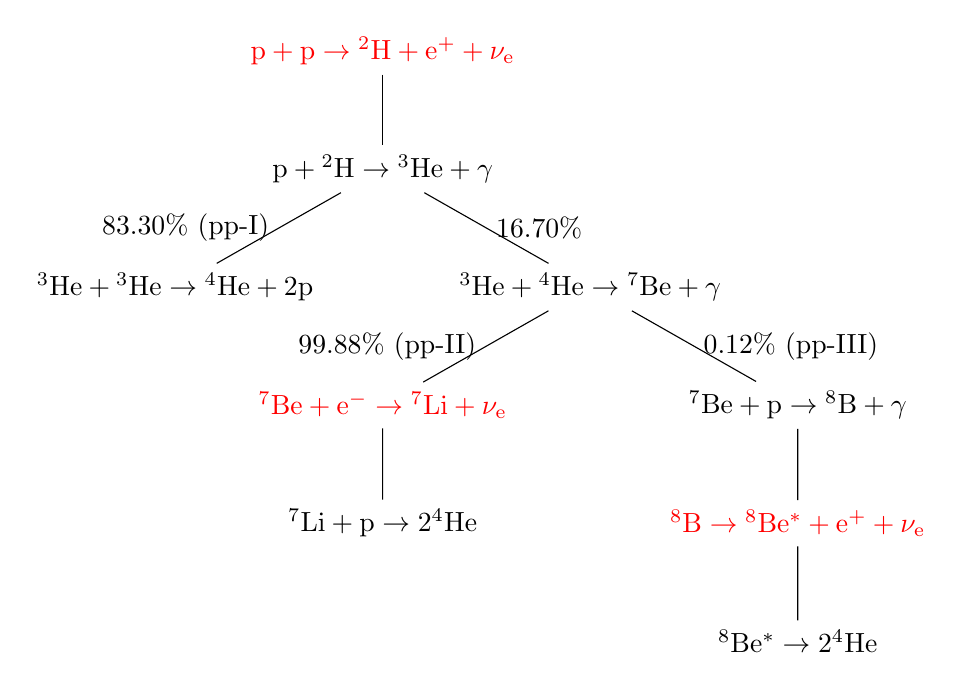
\begin{tikzpicture}[sibling distance=15em,
  every node/.style = {shape=rectangle,
    draw, align=center}
  edge from parent/.style = {draw, -latex},]]
  \node {\color{red}$\mathrm{p+p\to {}^2H + e^+ +\nu_e}$ }
    child { node {$\mathrm{p+{}^2H \to {}^3He + \gamma}$}
      child { node {$\mathrm{{}^3He+{}^3He \to {}^4 He + 2p }$}
          edge from parent node [left] {83.30\% (pp-I) } }
      child { node {$\mathrm{{}^3He+{}^4He \to {}^7 Be + \gamma }$}
        child { node { 
\color{red}$\mathrm{{}^7Be + e^- \to {}^7Li + \nu_e}$  
        }
        child { node { $\mathrm{{}^7Li + p \to 2{}^4He }$} }
        edge from parent node [left] {99.88\% (pp-II) } }
        child { node { $\mathrm{{}^7 Be + p \to {}^8 B + \gamma}$}
        child { node { \color{red}$\mathrm{{}^8B \to {}^8Be^* +e^+ +\nu_e}$ }
		child { node { $\mathrm{{}^8Be^* \to 2 {}^4He }$ } }}
        edge from parent node [right] {0.12\% (pp-III) } }
        edge from parent node [right] {16.70\%  } }};
\end{tikzpicture}
\end{adjustbox}
\caption{ pp chain with branching ratio. This is a modified version of Fig.~2 in \cite{Altmann2001} by Michael Altmann et al. }
\label{fig:pp_Chain_Branching}
\end{figure*}


% \begin{figure}[!hbtp]
% \centering
% 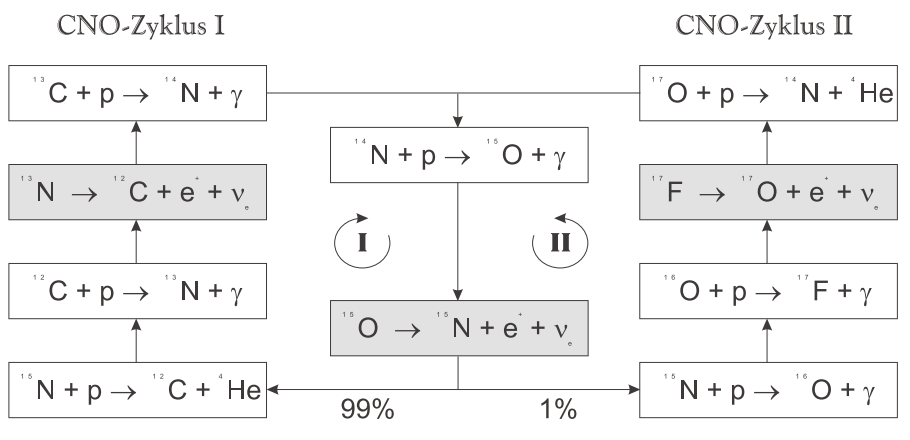
\includegraphics[width=\columnwidth]{chapters/assets/solar/cno_cycle.png}
% \caption{CNO cycle illustration~\cite{Adelberger2011a}.}
% \label{fig:cno_cycle}
% \end{figure}


Solar neutrinos are mostly produced in pp reaction, Be electron capture and B decay, which are called pp neutrinos, Be neutrinos and B neutrinos respectively. Even without knowledge of the detailed reactions, the conservation of lepton numbers will lead to the overall neutrino production
\begin{equation}
\mathrm{4p+2e^- \to {}^4He + 2\nu_e },
\end{equation}
where it is important to notice that two neutrinos are produced in each reaction. This overall reaction can either be pp chain or CNO cycle.

Using this simple relation, we can estimate the neutrino flux emitted by our sun. Given the kinetic energy produced in each reaction is the difference between the initial masses and the final masses, $Q_{pp}=4m_p+2m_e-m_{He4}=26.7\mathrm{MeV}$ where the mass of neutrinos are neglected since they are small compared with every other particle. On average, each neutrino carries away $0.2\mathrm{MeV}$ energy and the rest will be mostly in the form of thermal energy $Q_\gamma=26.3\mathrm{MeV}$~\cite{Adelberger2011a}. Number flux of thermal photons near Earth can be calculated using the solar constant $S_0$,
\begin{equation}
\Phi_\gamma = \frac{S_0}{Q_\gamma}.
\end{equation}
Since we know each reaction produces 2 neutrinos while producing $Q_\gamma$, which means that the number flux of neutrinos near Earth is roughly twice of the number flux of photons, i.e.,
\begin{equation}
\Phi_\nu = 2 \Phi_\gamma \approx 6\times 10^{10} \mathrm{cm^{-2}s^{-1}}.
\end{equation}
For such a large flux, understanding the role in stellar nuclear reaction and spectra is important.

Inside our Sun, two additional reactions also produce neutrinos which are called pep and hep neutrinos.
\begin{itemize}
\item pep neutrinos are produced in 
\begin{equation}
\mathrm{p + e^- + p \to {}^2H +\nu_e},
\end{equation}
which is only has a branching ratio 0.4\% instead of the 99.6\% of pp reaction.
\item hep neutrinos are produced in
\begin{equation}
\mathrm{ {}^3He + p \to {}^4He + e^+ \nu_e },
\end{equation}
which has a branching ratio of $2\times 10^{-5}\%$. As a comparison, the $\mathrm{{}^3He + {}^3He}$ has a branching ratio $85\%$ and $\mathrm{{}^3He + {}^4He}$ has a branching ratio $15\%$.
\end{itemize}


\section{\label{chap:basics-sec:vacuum-osc}Neutrino Oscillations in Vacuum}

Neutrinos are special particles that their flavor eigenstates are not the propagation eigenstates, which leads to neutrino flavor conversions while they propagate. Since neutrinos with different flavor interact with matter with different cross section, we need to investigate the neutrino flavor carefully. Even though only electron flavor neutrinos are produced, what we detect on Earth is different in flavor, which depends on two phenomena, neutrino vacuum oscillation and Mikheyev–Smirnov–Wolfenstein effect.


To understand the neutrino vacuum oscillations phenomenon, we use two-flavor neutrinos scenario as an example\footnote{In most physical problem, two-flavor scenario is a good approximation. The mass splits between the three mass eigenstates are very different so that the oscillation scales differ a lot for the different mass splits. Qualitatively speaking, the two-flavor scenario captures the significant features of the corresponding mass split.}.

Before we work out the math, we estimate the frequency of the interchange between flavors. With the natural units system, frequency is of dimension energy, see Appendix~\ref{chap:app-sec:conventions-subsec:units}. We also notice that energy of the particle,
\begin{align}
E_i^{(v)} & = \sqrt{m_i^2 + p_i^2 } \\
& = p_i \sqrt{\frac{m_i^2}{p_i^2} + 1} \\
& \approx p_i + \frac{1}{2} \frac{m_i^2}{p_i},
\label{chap:basics-section:neutrinos-eqn:energy-taylor}
\end{align}
is the only energy scale in this problem. The reason that we kept the second order in Taylor expansion is that we are interested in the different of energies between different mass eigenstates. We assume the neutrinos have almost the same momentum, which is true since their mass is small, i.e., $p_i \approx E$. Overall constant energy of free particles in quantum mechanics provides a global phase, which we are not interested in. So the only energy scale in our problem is the difference of energies between the two mass eigenstates, $\frac{\delta m^2}{2E}$. The frequency of flavor oscillations should be
\begin{equation}
    \omega \sim \frac{\delta m^2}{2E}.
    \label{chap:basics-section:neutrinos-eqn:qualitative-method-frequency}
\end{equation}
We'll show that this is indeed the frequency.

To work out the exact solutions, we utilize the Schr\"{o}dinger equation. The wave function in flavor eigenstates basis is related to wave function in mass eigenstates through an unitary matrix $\mathbf U$,
\begin{equation}
\Psi_{v}^{(f)} = \mathbf{U}_{v}\Psi_{v}^{(v)},
\end{equation}
where $\Psi_{v}^{(f)}$ is the wave function in flavor basis and $\Psi_{v}^{(v)}$ is the wave function in vacuum mass eigenstate basis. Upper index ${}_{v}$ is used to denote vacuum oscillations. The rotation matrix is
\begin{equation}
\mathbf{U}_{v} = \begin{pmatrix} \cos\theta_v & \sin \theta_v \\ -\sin \theta_v & \cos \theta_v \end{pmatrix}.
\end{equation}
In vacuum basis, the Hamiltonian is free propagation, which is given by
\begin{equation}
H_v^{(v)} = \begin{pmatrix} E_1 & 0 \\
0 & E_2
\end{pmatrix},
\end{equation}
where $E_i$ is defined in Eqn.~\ref{chap:basics-section:neutrinos-eqn:energy-taylor}.
To first order, the Hamiltonian becomes
\begin{align*}
H_v^{(v)} &= \frac{1}{2E} \begin{pmatrix}
m_1^2 & 0 \\
0 & m_2^2
\end{pmatrix} + E \mathbf{I}\\
& =  \frac{1}{4E} \begin{pmatrix}
m_1^2 - m_2^2 & 0 \\
0 & m_2^2 - m_1^2
\end{pmatrix} \\
&\phantom{=}+ \frac{m_2^2 + m_1^2}{4E} \mathbf{I} + E \mathbf{I},
\end{align*}
where the identity matrices only give us an overall phase so we drop them. With the definition that $\delta m^2 = m_2^2 - m_1^2$ The vacuum Hamiltonian in mass basis is simplify
\begin{equation}
H_v^{(v)} =  \frac{\delta m^2}{4E} \begin{pmatrix}
-1 & 0 \\
0 & 1
\end{pmatrix} = -\frac{\delta m^2}{4E} \sigma_3 = -\frac{\omega_{v}}{2}\sigma_3 ,
\end{equation}
which leads to the simple solution for the wave function in mass basis
\begin{equation}
\Psi_v^{(v)}(t) = \begin{pmatrix}
c_1(0) e^{i \omega_v t/2 } \\
c_2(0) e^{ -i\omega_v t/2 } 
\end{pmatrix}.
\end{equation}
% where the initial condition is
% \begin{equation}
% \Psi_v^{(v)}(0) = \begin{pmatrix}
% c_1(0) \\
% c_2(0) 
% \end{pmatrix}.
% \end{equation}
In flavor basis, the wave function at anytime is related to wave function in mass basis,
\begin{align}
\Psi_v^{(f)}(t) &= \mathbf{U}_v\Psi_v^{(v)}(t) \\
& = \begin{pmatrix} \cos\theta_v & \sin \theta_v \\ -\sin \theta_v & \cos \theta_v \end{pmatrix} \begin{pmatrix} c_1(0) e^{i\omega_v t/2 } \\
c_2(0) e^{ -i\omega_v t/2 }    \end{pmatrix} .
\end{align}

In many astrophysical neutrino sources such as the solar core, electron neutrinos are most abundant. Thus initial condition is usually assumed to be electron flavor in the calculation which leads to the survival probability of electron flavor
\begin{equation}
P(\nu_e,t) = \Psi_v^{(f)}(0)^\dagger \Psi_v^{(f)}(t) = 1-\sin^2(2\theta_v)\sin^2\left( \frac{\omega_v t}{2} \right).
\end{equation}
Since neutrinos travel with velocity approximately the speed of light, we use $L = t$ where $L$ is the distance travelled. The survival probability is
\begin{equation}
P(\nu_e,L) =  1-\sin^2(2\theta_v)\sin^2\left( \frac{\omega_v}{2} L \right).
\end{equation}
The important parameter is the oscillation length of the neutrino flavor conversion, $1/\omega_v$. This confirms our qualitative method result Eqn.~\ref{chap:basics-section:neutrinos-eqn:qualitative-method-frequency}. This result plotted in fig.~\ref{chap:basics-section:neutrinos-fig:vacuum-2-flavor-osc}, which clearly shows the oscillatory behavior. The oscillation length is determined by characteristic energy scale $\omega_v$, while the oscillation amplitude is determined by $\sin^2(2\theta_v)$.

Alternatively, we can find out the Hamiltonian in flavor basis first then solve the Sch\"{o}dinger equation. I will not show the steps here. However, the Hamiltonian in flavor basis is calculated for future use,
\begin{equation}
H_v^{(f)} = -\frac{\omega_v}{2}\cos 2\theta_v \sigma_3 + \frac{\omega_v}{2} \sin 2\theta_v \sigma_1.
    \label{chap:basics-sec:vacuum-osc-eqn:hamiltonian-vacuum}
\end{equation}

As for three flavor mixing, we have two quite different characteristic energy scales, $\omega_{v,21}=\delta m_{21}^2/2E$ and $\omega_{v,32}=\delta m_{31}^2/2E$. Thus two oscillation periods should occur, as shown in fig.~\ref{chap:basics-section:neutrinos-fig:vacuum-3-flavor-osc}. The fast oscillations are determined by the larger characteristic energy scale, $\omega_{v,32}$, while the slow oscillations are determined by the smaller one $\omega_{v,21}$. For inverted hierarchy, the oscillation frequencies are the same as normal hierarchy since they have the same characteristic energy scales. However ever they develop different oscillation phases.


\begin{figure}
    \centering
    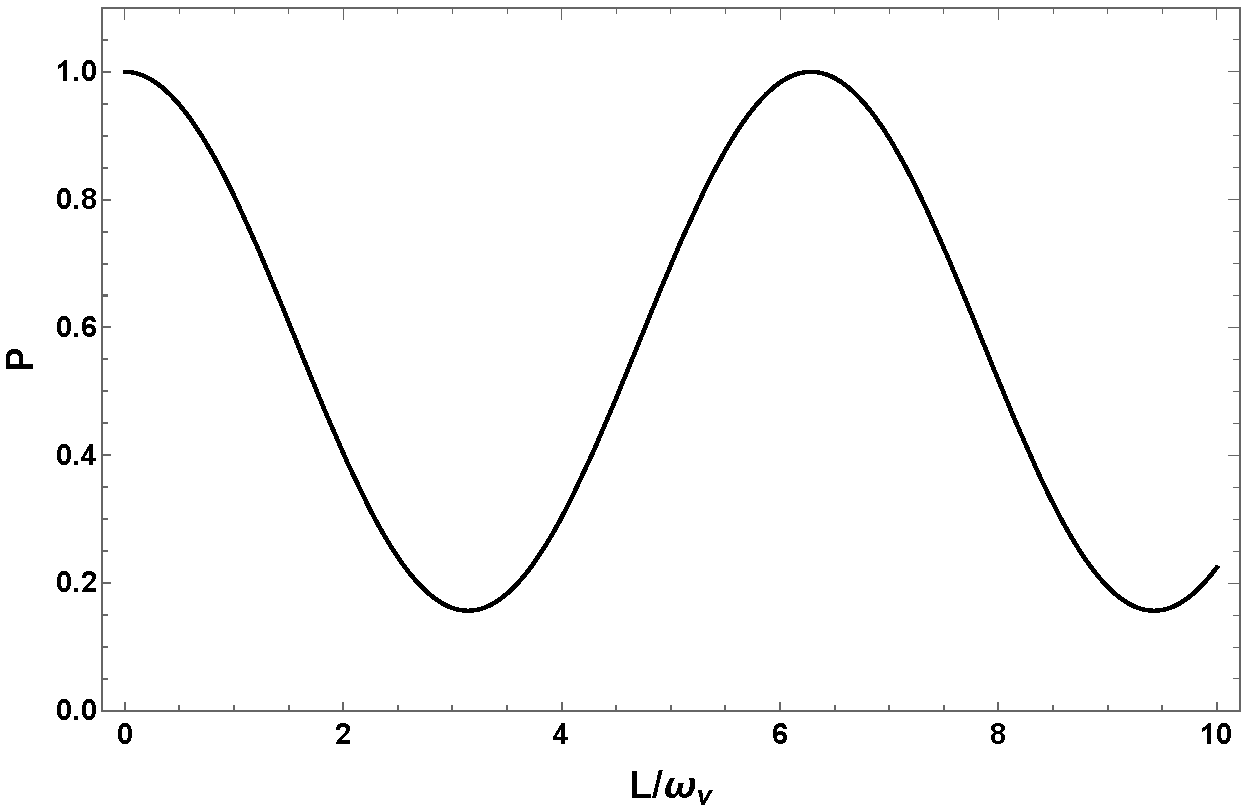
\includegraphics[width=\textwidth]{chapters/assets/basics/neutrino-vaccum-osc-2-flavor.pdf}
    \caption{Electron flavor neutrino survival probability in vacuum oscillations in two flavors scenario. Mixing angle is determined by $\sin^2\theta_{12}=0.30$.}
    \label{chap:basics-section:neutrinos-fig:vacuum-2-flavor-osc}
\end{figure}


\begin{figure}
    \centering
    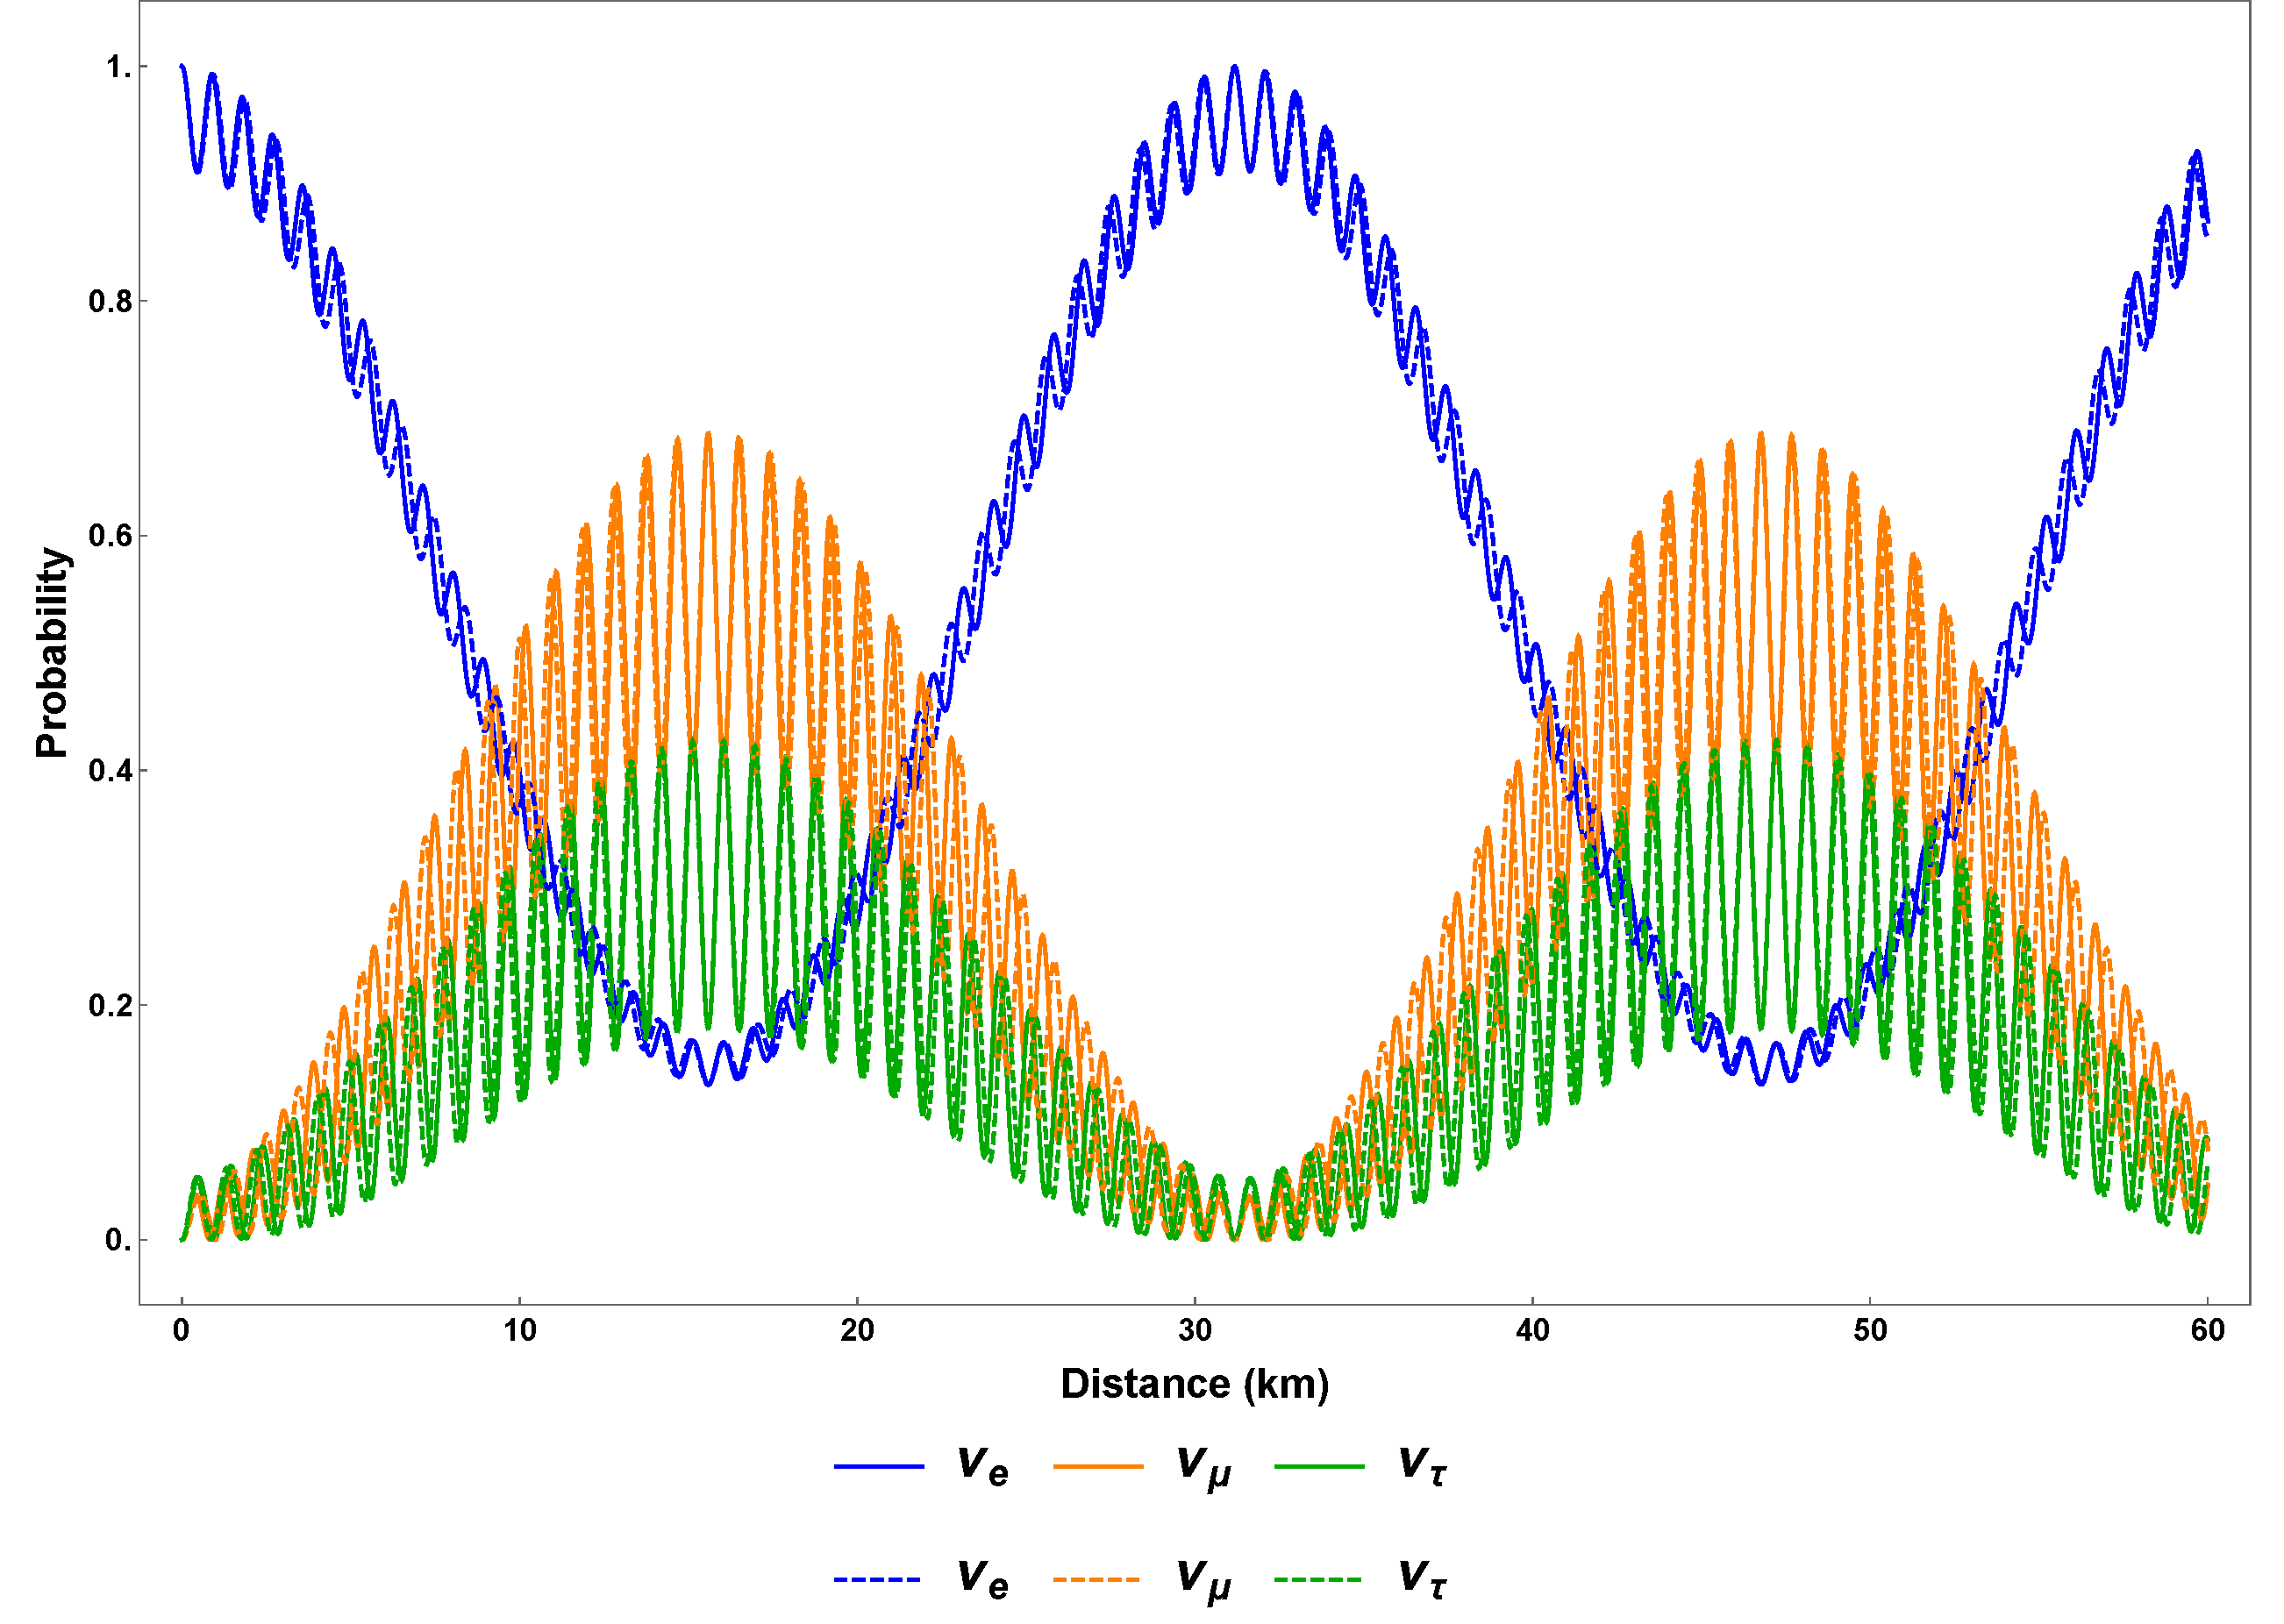
\includegraphics[width=\textwidth]{chapters/assets/basics/vacuum-oscillations-3-flavor.pdf}
    \caption{Neutrino vacuum oscillations with three flavors. The solid lines represent normal hierarchy and the dashed lines represent inverted hierarchy. Mixing angles are determined by $\sin^2\theta_{12}=0.30$, $\sin^2\theta_{13}=0.023$, $\sin^2\theta_{23}=0.41$, while the mass differences are set to $\delta m_{21}^2 = 7.9\times 10^{-5}\mathrm{eV}$, $\delta m^2_{23}=2.7\times 10^{-3}\mathrm{eV}$. Energy of neutrinos is 1MeV.}
    \label{chap:basics-section:neutrinos-fig:vacuum-3-flavor-osc}
\end{figure}





\section{\label{chap:basics-sec:msw}Mikheyev - Smirnov - Wolfenstein Effect}

The nature of neutrino oscillations means that flavor conversion occurs as long as their propagation eigenstates are not flavor eigenstates. As neutrinos travel from the center of the star throughout to the surface, we expect neutrino propagation eigenstates in such matter background to be different from flavor states in general~\cite{wolf78}. Using the fact that neutral current interactions between different flavor neutrinos and matter is independent of flavor, we only include the charged current, which will produce a effective potential for electron flavor that is different for other flavors. In flavor basis, the effective potential is
\begin{equation}
V=\frac{\sqrt{2}G_{\mathrm F} n_{\mathrm e} }{2} \sigma_3,
\end{equation}
where $G_{\mathrm F}$ is Fermi constant, $n_{\mathrm e}$ is number density of electrons. We also removed the terms that is proportional to identity in this potential since it doesn't change the probability for flavors. The Hamiltonian with matter effect is the combination of vacuum oscillation and matter effect, which is, in flavor basis,
\begin{equation}
H_m = \frac{ \omega_v }{2}\begin{pmatrix} -\cos 2\theta_v & \sin 2 \theta_v \\ \sin 2\theta_v & \cos 2\theta_v  \end{pmatrix} + \frac{\sqrt{2}G_F n_e}{2} \sigma_3,
\end{equation}
where we used the result of flavor basis vacuum oscillation Hamiltonian
\begin{align}
H_v^{(f)}& = \mathbf{U} H_v^{(v)}\mathbf{U^\dagger} \\
&= \frac{ \omega_v }{2}\begin{pmatrix} -\cos 2\theta_v & \sin 2 \theta_v \\ \sin 2\theta_v & \cos 2\theta_v  \end{pmatrix}.
\end{align}
Utilizing Pauli matrices and the so called matter potential $\lambda = \frac{\sqrt{2}G_F n_e}{2}$, it is rewritten as
\begin{equation}
H_m = \left(\frac{\lambda}{2} -\frac{ \omega_v }{2} \cos 2\theta_v \right) \boldsymbol{\sigma}_3  + \frac{ \omega_v }{2} \sin 2\theta_v \boldsymbol{\sigma}_1.
\label{chap:basics-sec:msw-eqn:hamiltonian-matter-effect}
\end{equation}
Due to the off-diagonal terms in the Hamiltonian, the system will experience oscillations in flavor. A resonance, i.e., maximum mixing, dominates the system when the diagonal terms becomes zero,
\begin{equation}
\frac{\lambda}{2} -\frac{ \omega }{2} \cos 2\theta_v  = 0,
\end{equation}
which gives us the MSW resonance condition.

The importance of matter effect to our understanding of solar neutrinos is that it modifies the oscillation, depending on the matter density profile. For a solar mass star, we have almost adiabatic evolution of the neutrinos, which means that the instantaneous eigenstates and eigenvectors of Hamiltonian is good enough for the time dependent Schr\"{o}dinger equation. 


For simplicity, we define the vacuum frequency and the 'hatted' dimensionless quantities
\begin{align}
\hat\lambda & = \frac{\lambda}{\omega_v}.
\end{align}
The eigenstates, derived by diagonalizing the Hamiltonian, are
\begin{align}
E_1 &= \frac{\omega_v}{2}\sqrt{ \hat\lambda +1 -  2\hat\lambda \cos 2\theta_v }\\
E_2 &= -\frac{\omega_v}{2}\sqrt{ \hat\lambda +1 -  2\hat\lambda \cos 2\theta_v }.
\end{align}


\begin{figure}
\centering
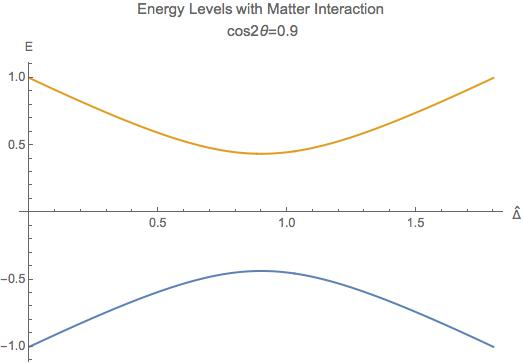
\includegraphics[width=0.7\columnwidth]{chapters/assets/solar/mswEnergyLevels.jpg}
\caption{The two energy levels in matter effect. The energy has unit $\omega_v/2$ while the potential has unit $\omega_v$. $\cos2\theta=0.9$ is applied.}
\label{fig:mswEnergyLevels}
\end{figure}

Fig.~\ref{fig:mswEnergyLevels} shows the two energy levels. For very high matter density, which interact with electron neutrinos more through charged current, electron flavor is composed almost with heavy propagation eigenstate. However, as the matter density becomes lower, the heavy propagation state will be gradually transformed to the other flavors since electron flavor in vacuum is composed mostly the light mass state. The resonance, which is the closest point of energy levels, happens at density $n_{\mathrm e} = 2\omega_v \cos(2\theta_v)/\sqrt{2}G_F$ which depends on $\omega_v$. Neutrinos with different energies have different resonance, which will significantly reshape the neutrino spectra for different flavors. 

One of the interesting fact about MSW effect is the MSW triangle shown in Fig.~\ref{chap:basics-sec:msw-fig:msw-triangle}. The survival probability of electron flavor neutrinos is plotted against $\log (\lambda/\omega_v)$ and $\log (\sin^2 2\theta_v)$. The low survival probability region is a triangle shape.
\begin{figure}
    \centering
    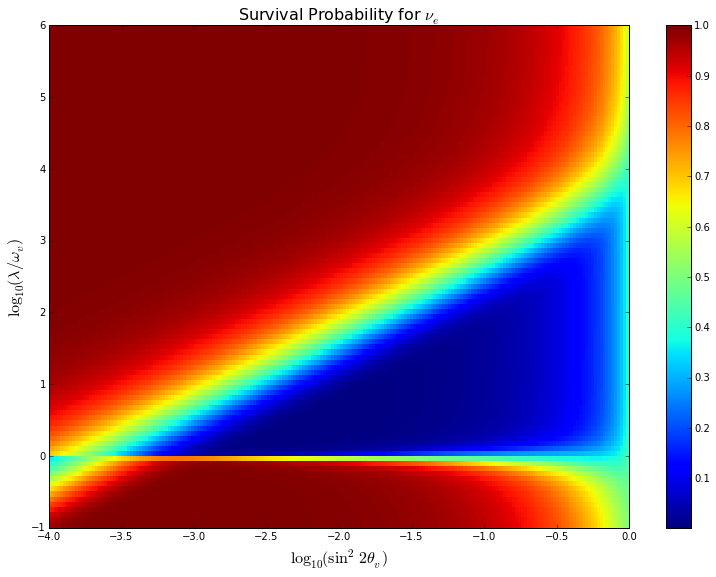
\includegraphics[width=0.9\textwidth]{chapters/assets/basics/msw-triangle.png}
    \caption{MSW triangle.}
    \label{chap:basics-sec:msw-fig:msw-triangle}
\end{figure}


In summary, even though only electron flavor neutrinos are produced in the core of a solar mass star, the neutrino flavor conversion to the other flavors is enhanced by matter interaction, in addition to the vacuum oscillation. However, the actual neutrino flavor conversion is much more complicated than just MSW effect and almost impossible to calculate without knowing the very exact matter profile of the Sun even with the time-dependent small perturbations to the density. As an approximation, MSW transition is good enough for the solar neutrinos~\cite{Lopes2013a}.


\section{\label{chap:basics-sec:flavor-isospin-pic}Flavor Isospin Picture of Neutrino Oscillations}

I explained neutrino oscillations in vacuum and the MSW effect in the previous sections. In principle, the oscillations in two flavor scenario are a consequence of the Hamiltonian in this quantum two level system. It's known that quantum two level systems are visualized using Bloch sphere. In the realm of neutrino physics, flavor isospin was introduced for such visualizations~\cite{Duan2006b}. The Hamiltonian for neutrino oscillations in vacuum (Eqn.~\ref{chap:basics-sec:vacuum-osc-eqn:hamiltonian-vacuum}) and in matter (Eqn.~\ref{chap:basics-sec:msw-eqn:hamiltonian-matter-effect}) can be reformulated into vector forms. 

We start with the vector form of Hamiltonian for vacuum oscillations. Mathematically speaking, we will cast every two by two matrix into the quaternian basis,
\begin{equation}
    H_v^{(f)} = - \frac{\vec{\boldsymbol{\sigma}} }{2}\cdot \vec H.
\end{equation}
Flavor isospin is defined as
\begin{equation}
    \vec s = \Psi^{\dagger} \frac{\vec{\boldsymbol{\sigma}} }{2} \Psi.
\end{equation}
As shown in Fig.~\ref{chap:basics-sec:flavor-isospin-pic-fig:flavor-isospin-illus}, the directions of flavor isospin tells us the flavor composite of neutrinos. In flavor isospin formalism, electron flavor survival probability is related to the third component of the flavor isospin,
\vspace*{0pt}
\begin{equation*}
P = \frac{1}{2} + s_3.
\end{equation*}
Correspondingly, equation of motion becomes precessions around the Hamiltonian,
\begin{equation}
\dot{\vec s} = \vec s \times \vec H.
\label{chap:basics-sec:flavor-isospin-pic-eqn:eom-precession}
\end{equation}
The precessions corresponds to periodic oscillations between flavors.

\begin{figure}
    \centering
    \vspace*{-10pt}
    \includegraphics[width=\textwidth]{chapters/assets/basics/flavor-isospin-illus}
    \caption{In flavor isospin picture, flavor isospin pointing upward indicates the neutrinos are in electron flavor, while the downward direction indicates the other flavor, such as muon flavor.}
    \label{chap:basics-sec:flavor-isospin-pic-fig:flavor-isospin-illus}
\end{figure}

We first work out the vacuum oscillations. Vacuum oscillation Hamiltonian becomes
\begin{align*}
&\frac{\omega_{\mathrm v} }{2}\left( - \cos 2\theta_{\mathrm v } \boldsymbol{\sigma}_3  + \sin 2\theta_{\mathrm{v}} \boldsymbol{\sigma}_1\ \right)
\to  \cos 2\theta_{\mathrm v}\begin{pmatrix}
0\\
0\\
\omega_{\mathrm v}
\end{pmatrix} -\sin 2\theta_{\mathrm v}\begin{pmatrix}
\omega_{\mathrm v}\\
0\\
0
\end{pmatrix}
\end{align*}
We assume neutrinos start with electron flavor, as explained in Sec.~\ref{chap:basics-section:astro}. Following the equation of motion Eqn.~\ref{chap:basics-sec:flavor-isospin-pic-eqn:eom-precession}, neutrinos precess around vector $\vec H$ that is tilted away from the vertical axis, as shown in Fig.~\ref{chap:basics-sec:flavor-isospin-pic-fig:flavor-isospin-vac-osc}. The oscillation frequency is trivially read out from the precession equation,
\begin{equation*}
    \omega_{\mathrm v} = \lvert \vec H_{\mathrm v} \rvert.
\end{equation*}


\begin{figure}
    \centering
    \vspace*{-20pt}
    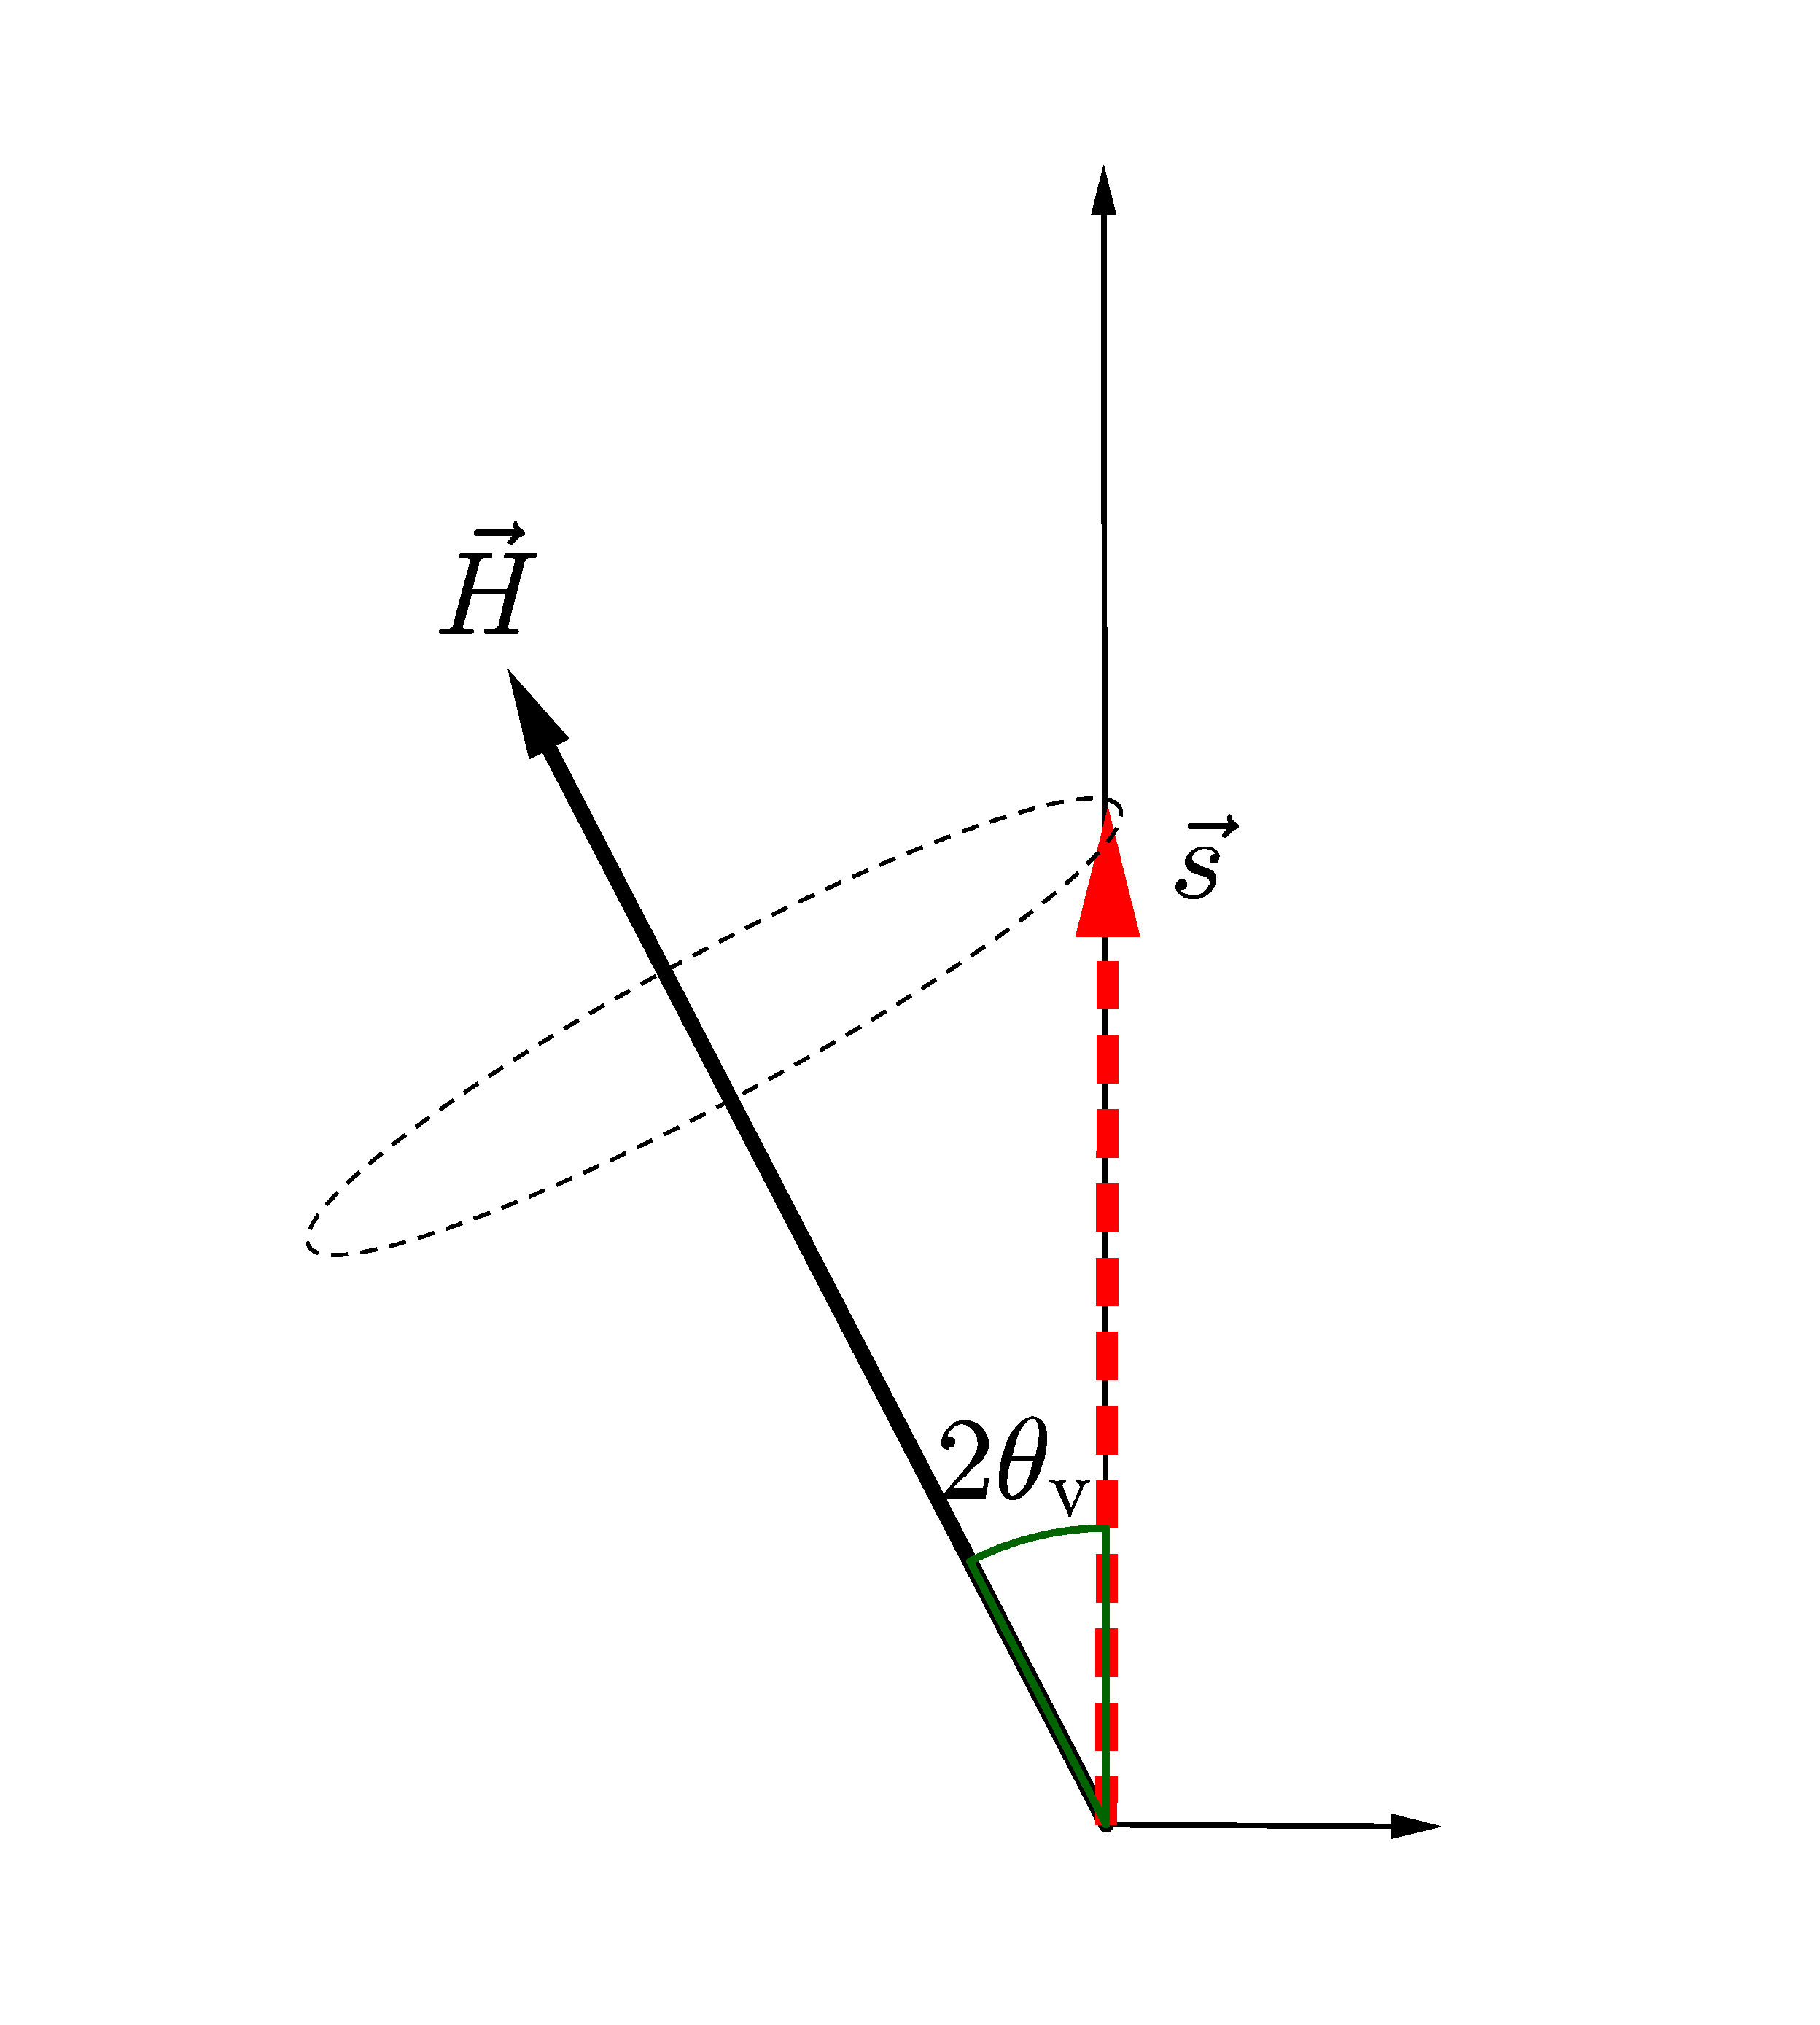
\includegraphics[width=0.7\textwidth]{chapters/assets/basics/flavor-isospin-vac-osc}
    \caption{Vacuum oscillations in flavor isospin picture. Neutrinos starting with electron flavor will follow a precession pattern around the static "Hamiltonian vector" $\vec H$, thus periodic flavor oscillations.}
    \label{chap:basics-sec:flavor-isospin-pic-fig:flavor-isospin-vac-osc}
\end{figure}


MSW effect is also easily explained using flavor isospin picture. The Hamiltonian in flavor isospin picture
\begin{align*}
    H_m =& \frac{\omega_{\mathrm{v}}}{2}\left( - \cos 2\theta_{\mathrm{v}} \boldsymbol{\sigma_3} + \sin 2\theta_{\mathrm{v}} \boldsymbol{\sigma_1} \right)   + \frac{\lambda(x)}{2} \boldsymbol{\sigma_3} \\
    \to &  \omega_{\mathrm v}\begin{pmatrix}
    - \sin 2\theta_{\mathrm v} \\
    0 \\
    \cos 2\theta_{\mathrm v}
    \end{pmatrix}   + \begin{pmatrix}
    0\\
    0\\
    - \lambda(x)
    \end{pmatrix}  \\
    = &  \vec H_{\mathrm v} + \vec H_{\mathrm m}(x),
\end{align*}
where $\vec H_{\mathrm v}$ is vacuum contribution and $\vec H_{\mathrm m}(x)$ is the matter potential contribution. The two vectors are visualized in Fig.~\ref{chap:basics-sec:flavor-isospin-pic-fig:matter-effect-notsolarge-density}. We discussed in Sec.~\ref{chap:basics-sec:msw} the adiabatic transitions of neutrino states in varying matter density. Fig.~\ref{chap:basics-sec:flavor-isospin-pic-fig:msw-adiabatic} shows the adiabatic evolution of neutrino flavor isospin. For region of high density matter background, which provides large matter potential, the total Hamiltonian is almost pointing downward. We observe almost no flavor oscillations since flavor isospin precession is tiny. As the neutrinos moving into smaller matter density regions, the flavor isospin is approximately following the evolution of Hamiltonian. Flavor conversion happens because of the evolution of Hamiltonian, even though flavor oscillations are still tiny. In the end, neutrinos reach the region with almost no matter, where they are almost converted to one of the mass eigenstates. In fact, those neutrinos won't oscillate that much in vacuum following this initial condition.



\begin{figure}[htbp]
    \centering
    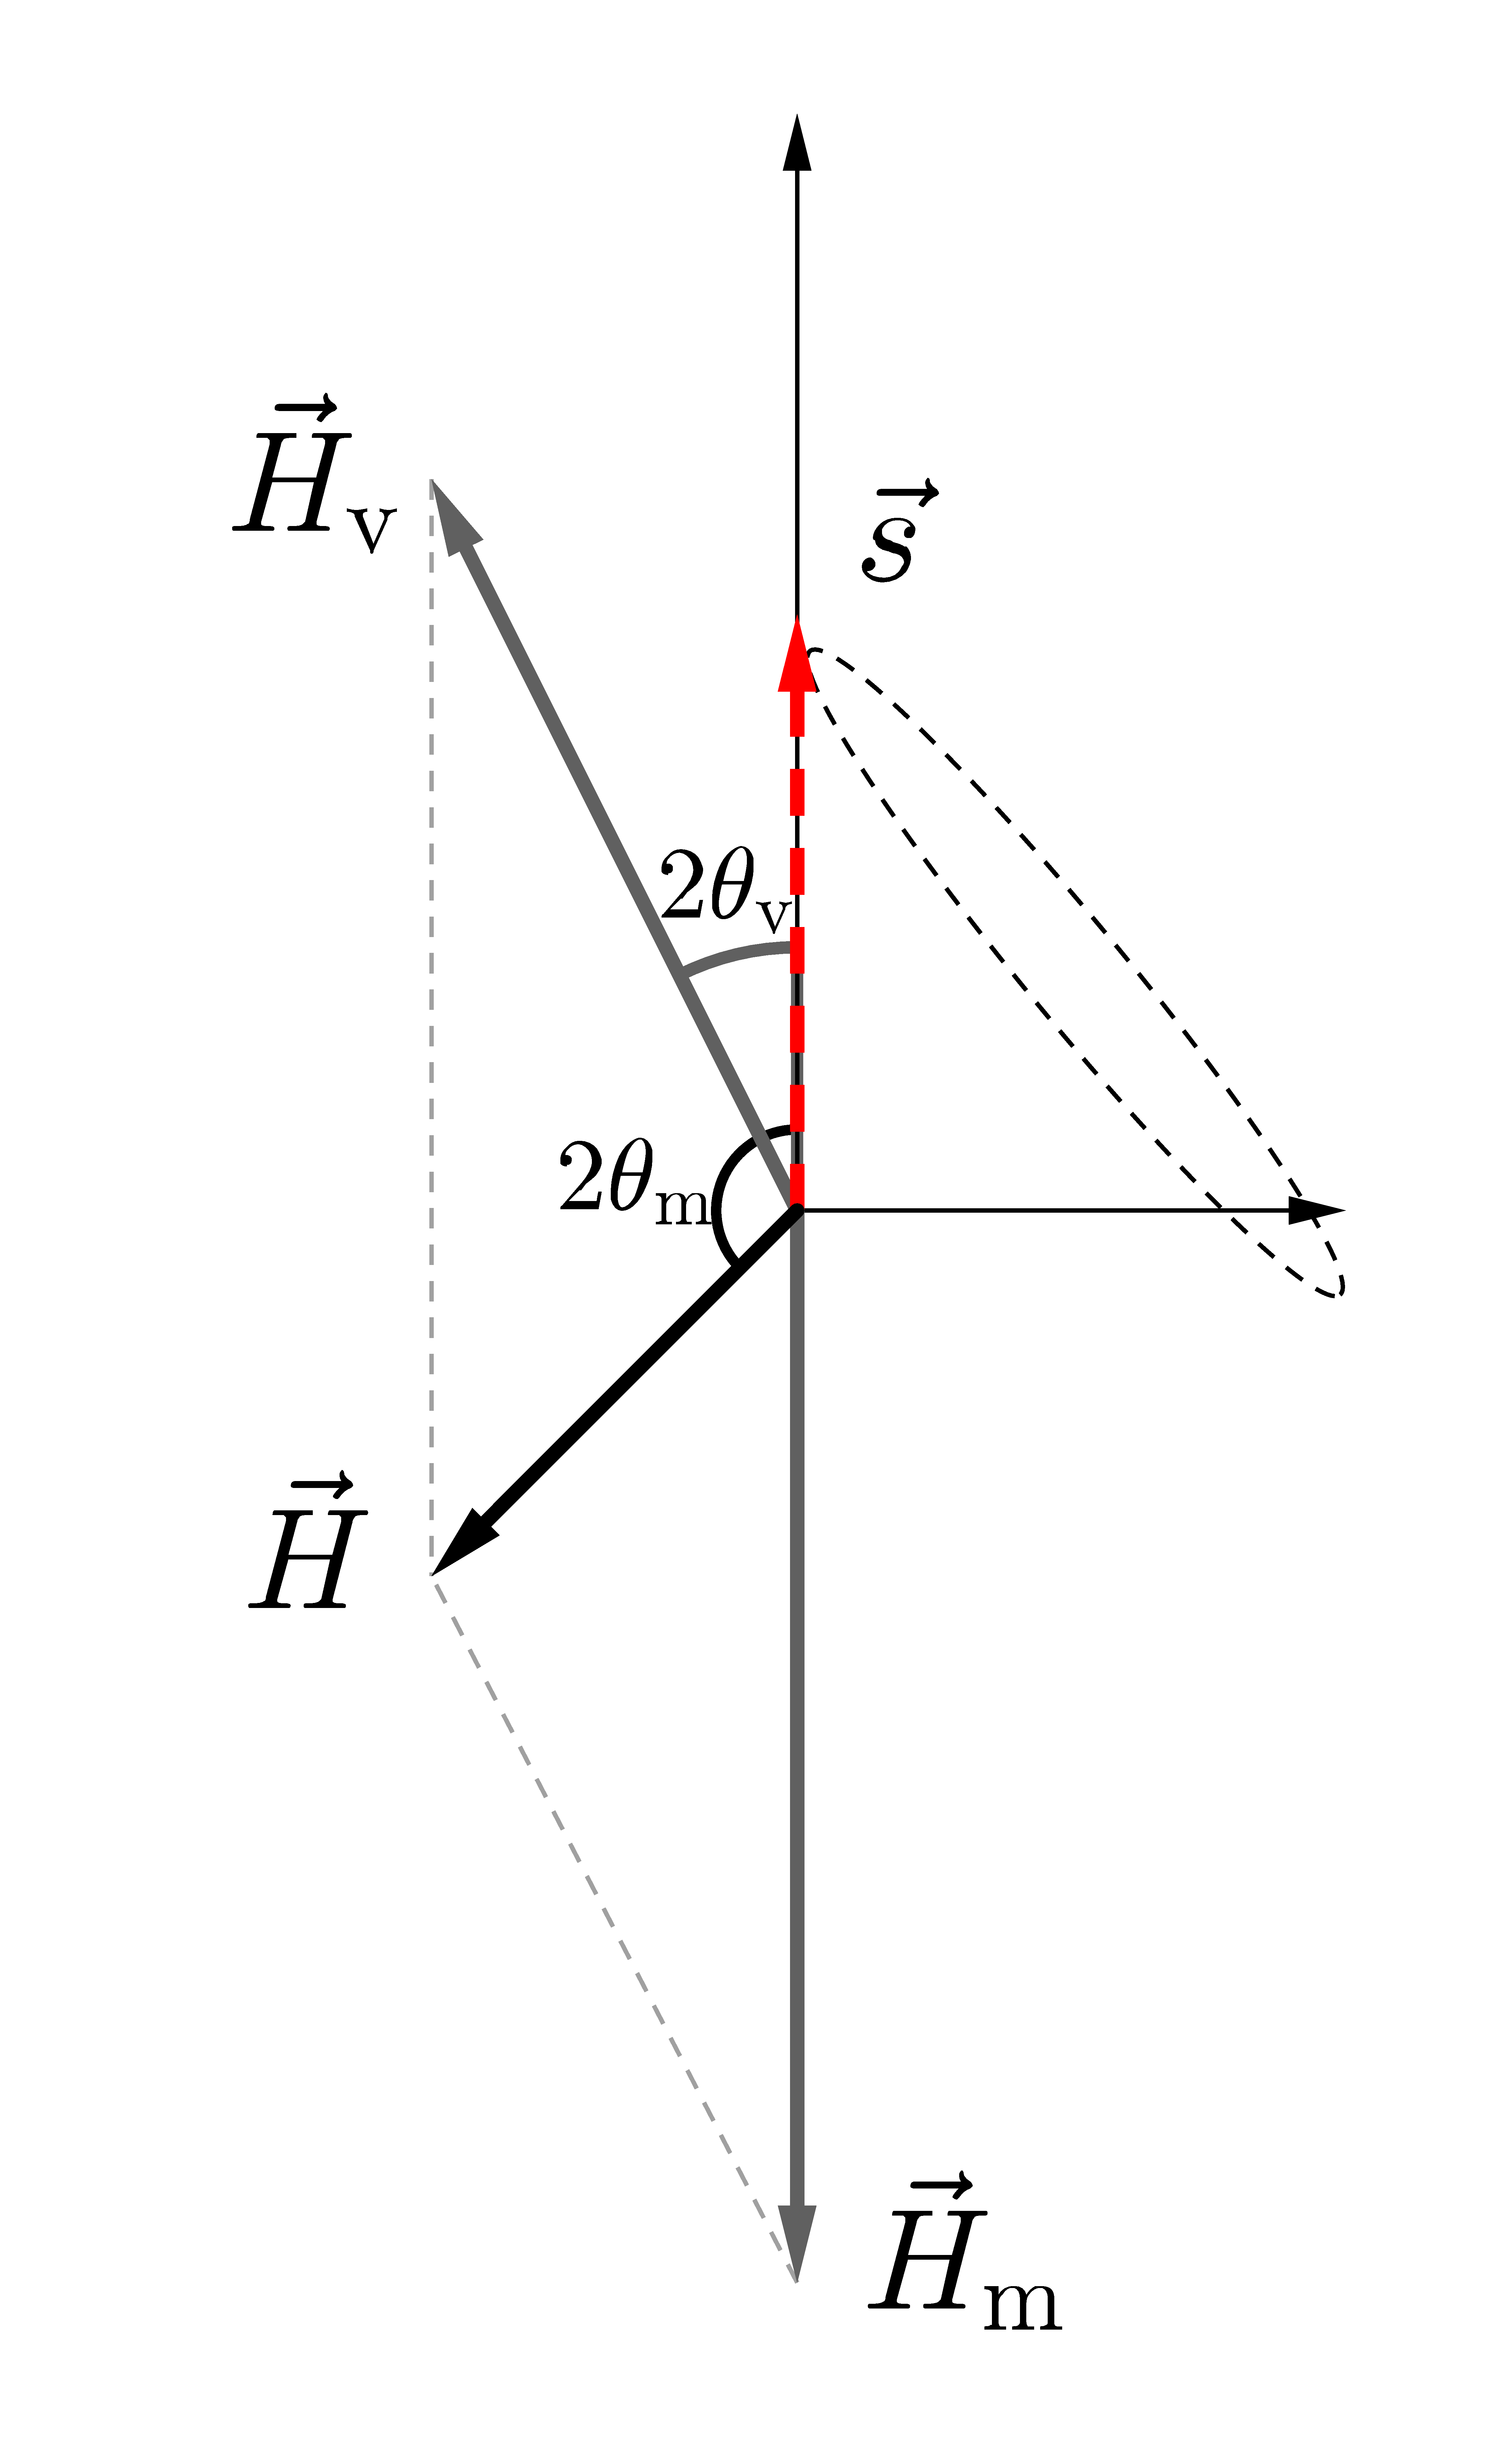
\includegraphics[width=0.5\textwidth]{chapters/assets/basics/matter-effect-notsolarge-density}
    \caption{}
    \label{chap:basics-sec:flavor-isospin-pic-fig:matter-effect-notsolarge-density}
\end{figure}




\begin{figure}[htbp]	
	\centering
	\begin{subfigure}[t]{0.3\textwidth}
		\centering
		\includegraphics[width=0.8\textwidth]{chapters/assets/basics/matter-effect-large-density}
		\caption{High matter density}\label{chap:basics-sec:flavor-isospin-pic-fig:msw-adiabatic-large-density}
	\end{subfigure}
	\quad
	\begin{subfigure}[t]{0.3\textwidth}
		\centering
		\includegraphics[width=0.8\textwidth]{chapters/assets/basics/matter-effect-adiabatic}
		\caption{Medium matter density}\label{chap:basics-sec:flavor-isospin-pic-fig:msw-adiabatic-medium-density}		
	\end{subfigure}
	\quad
	\begin{subfigure}[t]{0.3\textwidth}
		\centering
		\includegraphics[width=0.8\textwidth]{chapters/assets/basics/matter-effect-adiabatic-small-density}
		\caption{Low matter density}\label{chap:basics-sec:flavor-isospin-pic-fig:msw-adiabatic-small-density}
	\end{subfigure}
	\caption{Flavor isospin picture of neutrino oscillations in matter. $\vec H_{\mathrm v}$ is the vacuum contribution to Hamiltonian, and $\vec H_{\mathrm m}$ corresponds to the matter potential.}\label{chap:basics-sec:flavor-isospin-pic-fig:msw-adiabatic}
\end{figure}

Neutrinos might experience a critical matter density, when the overall Hamiltonian is perpendicular to the upright axis. Assuming we have electron neutrinos going through such regions, they will experience maximum flavor oscillations, c.f.~Fig.~\ref{chap:basics-sec:flavor-isospin-pic-fig:msw-adiabatic-critical}.

\begin{figure}
    \centering
    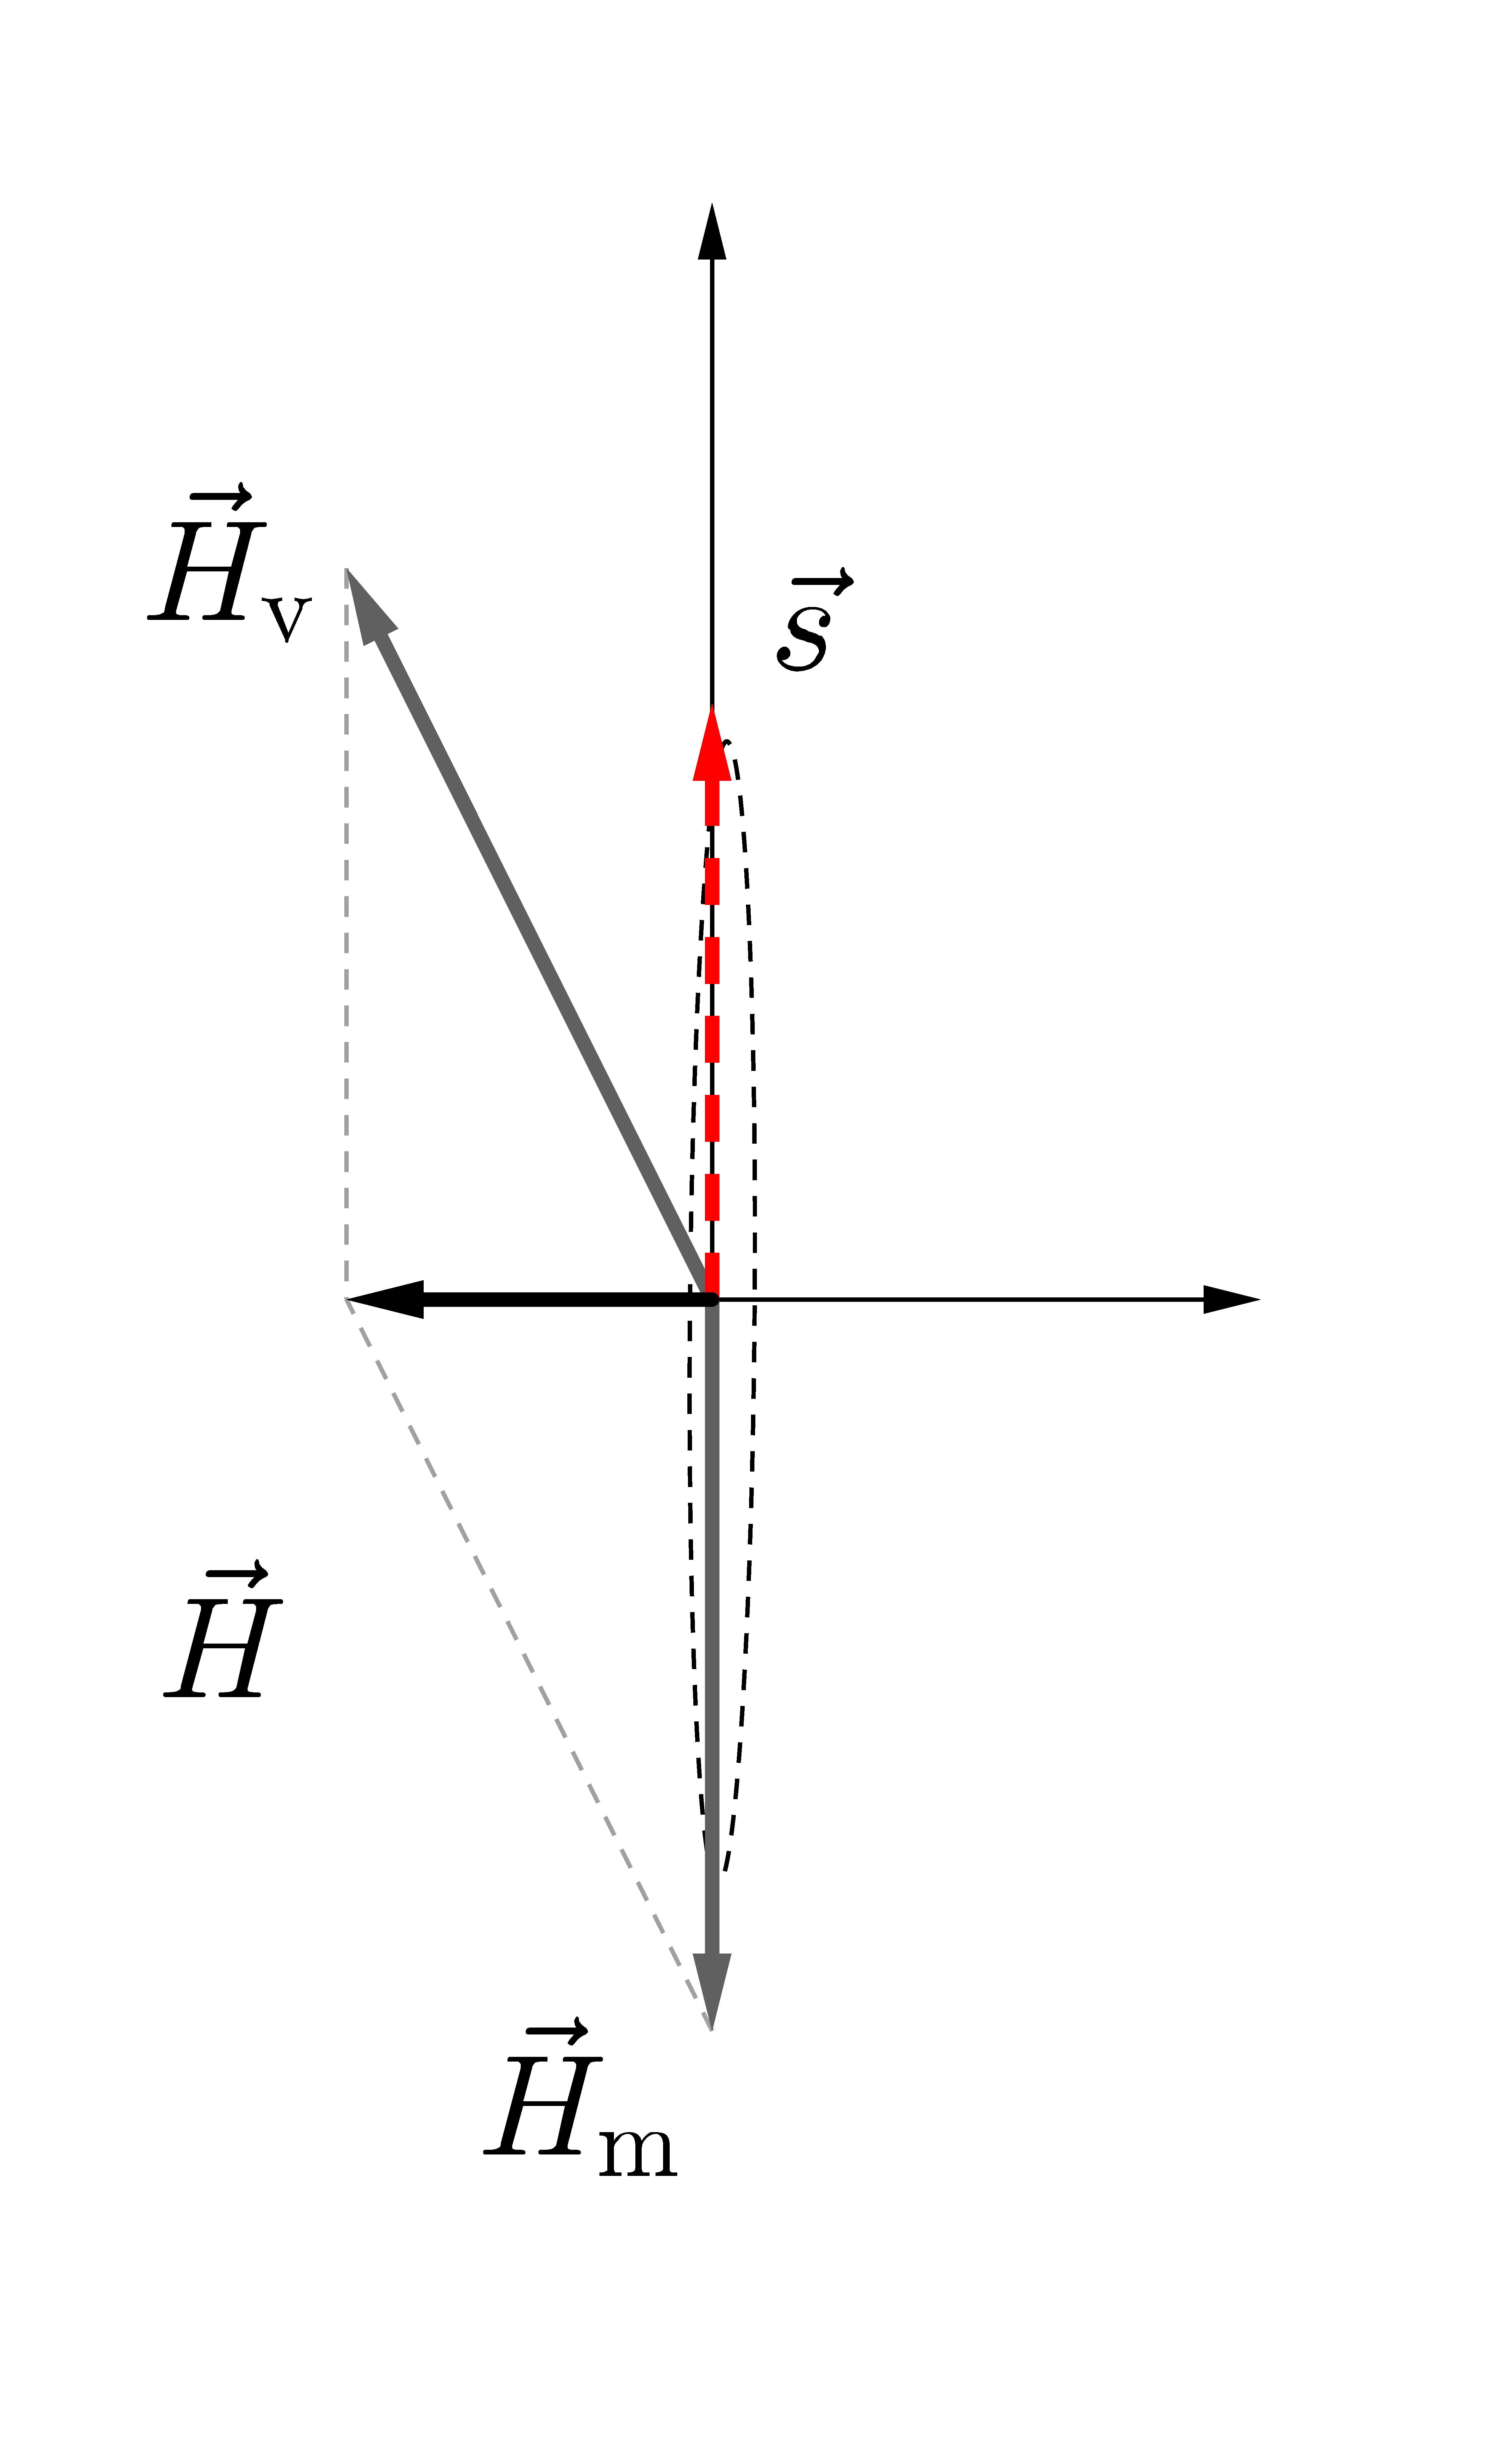
\includegraphics[width=0.5\textwidth]{chapters/assets/basics/matter-effect-critical-density}
    \caption{MSW resonance happens when electron neutrinos go through a critical matter density.}
    \label{chap:basics-sec:flavor-isospin-pic-fig:msw-adiabatic-critical}
\end{figure}




\section{Supernova Neutrinos and Conclusion}


The solar neutrinos behave very differently from lab experiments since the Sun provides a high matter density lab which can not be built on the Earth. What's even more exotic, in a supernova explosion, $10^{58}$ neutrinos are released from the proto-neutron star, which is of radius $10\mathrm{km}$, in a few seconds. The huge number density of neutrinos and large density of matter both change the neutrino oscillations dramatically. The matter effect in supernova is also much more complicated than MSW for solar neutrinos since the rich distribution of matter density and high speed motion. In addition to matter effect, neutrino neutrino interaction will be very efficient because of the high neutrino number density.

Apart from the emission of neutrinos from nuclear reactions of electron capture and positron emission in the solar interior, supernova environment also gives rise to Bremsstrahlung pair neutrino production, electron-positron neutrino pair production, which brings all three flavors and also anti-neutrinos into the spectra. However, even the with the presence of intensive interaction between neutrinos and the leptons and hardrons, which thermalize the neutrinos in the supernova core, the neutrino spectrum escaping from the supernova core is not completely Fermi-Dirac distribution. Nonetheless, it is possible to parametrize it using nominal Fermi-Dirac distribution,\cite{ysuzuki2004}
\begin{equation}
f(E)\propto \frac{E^2}{1+\exp ( E/kT - \mu )}.
\end{equation}
Some numerical results show that there is a deviation from this Fermi-Dirac distribution~\cite{Totani1998,Keil2003}. Meanwhile, Keil Mathias and Georg Raffelt showed that it is good enough to approximate the neutrino spectrum from supernova in Monte Carlo simulations using the so called "alpha fit",
\begin{equation}
f(E)\propto E^\alpha \exp\left( -(\alpha+1)\frac{E}{\langle E\rangle} \right),
\end{equation}
where $\langle E\rangle$ is the average energy, or the first moment of energy. The values from Monte Carlo simulations falls into the range $\alpha = 2.5\sim 5$,
which clearly shows the spectra are pinched. It's a hint that the detection of deviation from nominal Fermi-Dirac distribution will show evidence of core-collapse information.


% \begin{figure}
% \centering
% 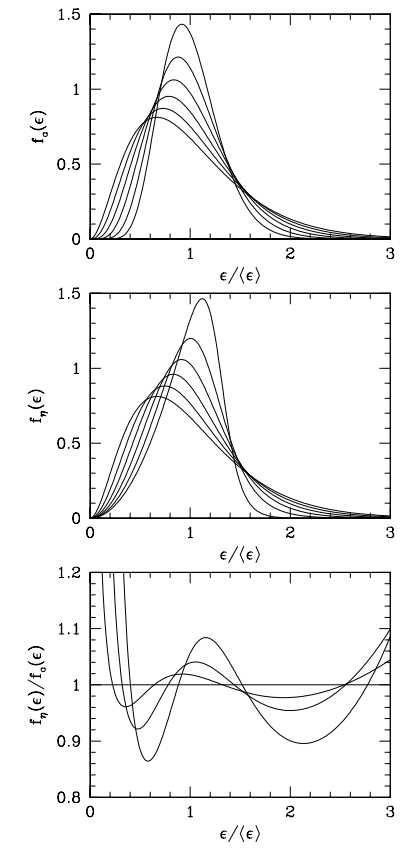
\includegraphics[width=\columnwidth]{chapters/assets/solar/neutrino_spectra_sn_simulations.png}
% \caption{Alpha fit and nominal Fermi-Dirac fit comparison. The top panel is alpha fit results while the middle panel is from nominal Fermi-Dirac distribution fit. The broadest curve are for $\alpha=2$. The width $w=\sqrt{\langle E^2 \rangle - \langle E\rangle^2}$ decrease 10\% for each curve. The bottom panel is the ratio of the two fit functions.}
% \label{fig:neutrino_spectra_sn_simulations}
% \end{figure}


Even though we understand solar neutrinos well, the neutrino oscillations of supernova explosions are not so to our complete knowledge. The flavor content is subject to the solution to the neutrino oscillations. Phenomena such as spectral split due to neutrino-neutrino interaction and matter effect reshape the neutrino spectra significantly. That being said, more research on supernova neutrinos, especially supernova neutrino oscillations is critical to understand supernova explosion mechanisms, as well as future observation of supernova neutrino data.



